\section{Extended related work}\label{app:related}
Figure~\ref{fig:timeline} is the setting every family in Table~\ref{tab:related} is placed against: the queries that confer a row's
importance arrive after the compression decision, so a statistic of observed
attention has nothing to observe at the moment it must choose.

\begin{figure}[H]
\centering
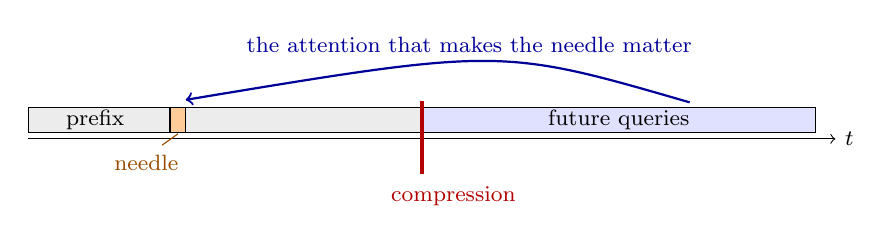
\begin{tikzpicture}[x=0.05cm,y=0.8cm,font=\footnotesize]
  \draw[->] (0,0) -- (205,0) node[right] {$t$};
  \draw[fill=gray!15] (0,0.10) rectangle (100,0.50);
  \draw[fill=orange!40] (36,0.10) rectangle (40,0.50);
  \draw[fill=blue!12] (100,0.10) rectangle (200,0.50);
  \node at (150,0.30) {future queries};
  \node at (17,0.30) {prefix};
  \node[orange!60!black,anchor=north] at (30,-0.10) {needle};
  \draw[orange!60!black] (34,-0.10) -- (38,0.08);
  \draw[very thick,red!70!black] (100,-0.55) -- (100,0.60);
  \node[red!70!black,anchor=north] at (108,-0.60) {compression};
  \draw[->,thick,blue!60!black] (168,0.58) .. controls (120,1.45) .. (40,0.62);
  \node[blue!60!black,anchor=south] at (112,1.22) {the attention that makes the needle matter};
\end{tikzpicture}
\caption{The needle's importance is conferred entirely by queries that do
not exist at compression time; H2O accumulates prefix attention, SnapKV
reads a window before the cut --- both see nothing
(Table~\ref{tab:baselines}).}
\label{fig:timeline}
\end{figure}


\begin{table}[H]
\centering\small
\caption{Who decides cache membership, and what their warm-up costs and
settles. The last column is why this method's warm-up cannot damage answers:
the archive is never deleted, so what a warm-up settles is re-settled every
step. Note the units of the warm-up cost, which differ per family --- training,
memory, prefill compute, or throughput --- and whether it grows with context.}
\label{tab:related}
\begin{tabular}{l>{\raggedright\arraybackslash}p{2.9cm}>{\raggedright\arraybackslash}p{4.6cm}l}
\toprule
family & selection signal & warm-up: cost $\to$ what it settles & deletes?\\
\midrule
trained sparse \citep{yuan-etal-2025-native,lu2025moba} & learned pattern &
 pre-training $\to$ the pattern itself & model changed\\
observed attention \citep{zhang2023h2oheavyhitteroracleefficient,NEURIPS2024_28ab4182,oren2024transformersmultistaternns,ICLR2024_5e5fd18f} &
 attention already seen & hold everything meanwhile, i.e.\ spend the very
 resource it exists to save $\to$ what to discard & yes\\
structural splits \citep{xiao2025duoattention,cai2024pyramidkv} &
 offline head/layer profile & offline $\to$ the per-head budget & yes\\
surrogate scoring \citep{kim2025kvzip} & reconstruction attention &
 ${\approx}2\times$ prefill, \emph{grows with context} $\to$ what to discard & yes\\
page digests \citep{tang2024questqueryawaresparsityefficient,chen2024arkvale} &
 per-page bound, looseness fixed statically & none --- bought by not adapting
 per request $\to$ nothing & yes\\
exact merging \citep{tian2025keepkvachievingperiodiclossless} & identical content &
 none $\to$ the merge class & class empty under RoPE\\
trained projection \citep{lin2025matryoshkakvadaptivekvcompression,gelberg2026trainingtransformerskvcache} &
 learned subspace & training $\to$ the projector & model changed\\
\textbf{VestigeKV} & vestigial branch; predates every query &
 ${\sim}18$ decode queries, \emph{flat in context}, paid in throughput $\to$
 how much to read back & \textbf{no}\\
\bottomrule
\end{tabular}
\end{table}

Two columns of Table~\ref{tab:related} carry the argument. The warm-up cost is
denominated differently in each family, and only here is it denominated in
something other than the resource being optimized: eviction that warms up by
holding everything spends memory to save memory, and surrogate scoring spends
prefill compute that grows with the context it is compressing, while this
method spends throughput and its warm-up is a fixed number of decode queries
regardless of context length. And what the warm-up settles is reversible only
here --- the archive is bit-exact and resident, so a row the provisional index
declines is reconsidered on the next step, where a row another method discards
during its warm-up is gone. The price of that reversibility is the $1.14\times$
cache of Section~\ref{sec:cost}: this method is not cheaper in memory, and the
comparison is honest only if that is read alongside the column.

Trained sparse attention \citep{yuan-etal-2025-native,lu2025moba} buys
content-aware patterns with pre-training; VestigeKV inherits its pattern
from a channel NoPE training has already repurposed, at zero cost.
Observed-attention eviction
\citep{zhang2023h2oheavyhitteroracleefficient,NEURIPS2024_28ab4182,oren2024transformersmultistaternns,ICLR2024_5e5fd18f} selects on
attention already seen; Section~\ref{sec:problem} measures that setting.
Structural splits precompute \emph{where} full cache is deserved
(retrieval vs.\ streaming heads \citep{xiao2025duoattention}, per-layer
pyramidal budgets \citep{cai2024pyramidkv}), but the per-token choice
inside the compressible part still reads observed attention. The closest prior occupant of the query-independent quadrant is
KVzip \citep{kim2025kvzip}, which scores each KV pair on RoPE models by the
attention it receives while the model reconstructs its own context. The
kinship is bounded on three axes: the signal there comes from surrogate
reconstruction queries at roughly twice the prefill cost, here it is read
off the cache at \readCost{} of row bytes with no forward pass; a
reconstruction score on a RoPE cache inherits the position drift of
Section~\ref{sec:math}(a), while the NoPE ranking is frozen at capture
(Corollary~\ref{cor:stationary}); and KVzip deletes, while the archive
here deletes nothing and re-admits rows per step under a certified trigger. Branch-differential studies
\citep{ma2026irminsulmlanativepositionindependentcaching,ma2026kameraunifiedpositioninvariantmultimodal} measure the \emph{rotated} branch
(branch-only AUC $0.43$); the unrotated case is measured here. ArkVale
\citep{chen2024arkvale} is the closest comparison: VestigeKV inherits its
evict-summarize-recall architecture, with four differences:
(i)~\emph{signal}: query-history page importance
vs.\ a query-independent signal that predates every query;
(ii)~\emph{granularity}: lossy page digests vs.\ row-level bit-exact
latents plus a 16-bit index;
(iii)~\emph{admission}: a top-$k$ page quota, which \emph{is} the admission
rule there, so a page past the quota is not recalled, vs.\ an uncapped
calibrated competition against the kept-tier maximum. Both cap the fetch, and
the cap is taken from this line of work; what differs is where it sits. Behind
the rule rather than inside it, an overflow has an exact destination --- the
full row set --- so the bound is spent in throughput instead of answers;
(iv)~\emph{certificate}: a digest bound valid only over the rotation
orbit (Table~\ref{tab:arkvale}) vs.\ the query-uniform Cauchy--Schwarz
bound of the fixed NoPE form, conformally calibrated at capture.
Page-bound selection \citep{tang2024questqueryawaresparsityefficient} inherits the same digest
obstruction; trained compression
\citep{lin2025matryoshkakvadaptivekvcompression,gelberg2026trainingtransformerskvcache} changes the model;
per-step exact merging under RoPE \citep{tian2025keepkvachievingperiodiclossless} is the strongest
possible there, and Proposition~\ref{prop:impossible} shows the query-universal version
needs NoPE$+$MLA. Architecture from \citep{deepseekai2024deepseekv2strongeconomicalefficient,kimiteam2025kimilinearexpressiveefficient}; NoPE's length-generalization case from
\citep{kazemnejad2023impactpositionalencodinglength,wang2024lengthgeneralizationcausaltransformers}.

\paragraph{Dividends inside prior algorithms.} Two facts of
Section~\ref{sec:math} --- one fixed bilinear score, and rankings that commute
with time --- restate several published cache policies once transplanted to
NoPE-MLA. They are derivations, not measurements, and three of them are
\emph{empty} on this checkpoint as measured. Appendix~\ref{app:dividends}
gives each one and its boundary.

